\chapter{Introduction}\label{chap:introduction}

% The central observation motivating this thesis is that axionlike particles (ALPs) interact with nuclear spins as an effective oscillating pseudomagnetic field.
% Nuclear magnetic resonance (NMR) is among the most sensitive techniques for detecting weak oscillating fields, making it a natural tool for direct ALP dark-matter searches.

Astrophysical evidence for dark matter comes from galaxy rotation curves, gravitational lensing, large-scale structure, and the cosmic microwave background: visible matter alone cannot account for the observed dynamics.
Axions and axionlike particles are theoretically attractive candidates because they are weakly coupled, naturally light, and can generate spin-precession signals accessible to NMR experiments.

This chapter introduces the key ingredients of the search.
Section~\ref{sec:intro:NMR} reviews the NMR concepts most relevant to the experiment.
Section~\ref{sec:intro:DM} summarizes the dark-matter evidence.
Section~\ref{sec:intro:axions} describes the axion and ALP framework, including the pseudomagnetic-field analogy that connects ALP physics to NMR.
Section~\ref{sec:intro:CASPEr} outlines the CASPEr project.
The theory of signal estimation and scanning optimization is developed in Chapter~\ref{chap:theory}; the apparatus is described in Chapter~\ref{chap:experiment}; measurements and results appear in Chapter~\ref{chap:results}.

\section{Nuclear magnetic resonance}\label{sec:intro:NMR}
Nuclear magnetic resonance is a technique for studying nuclear spins in magnetic fields.
In the presence of a bias magnetic field, spin states split by the Zeeman effect, resulting in nuclear polarization. 
A polarized sample acquires a non-zero net magnetization that precesses at the Larmor frequency.
Because the Larmor frequency is proportional to the magnetic field, NMR can be a tool for magnetic field measurement.

% The properties most relevant to this thesis are sensitivity to weak fields, applicability from zero to very high field, and a rich time-domain response.
% These allow axionlike spin precession to be treated as a small perturbation on a standard NMR experiment.

\subsection{Zeeman splitting and polarization}\label{sec:intro:NMR:Zeeman}
In a bias magnetic field $B_0$, a spin-$1/2$ nucleus splits into two energy levels separated by
\begin{equation}
    \Delta E = \hbar \gamma B_0
    \,,\label{eq:Zeeman}
\end{equation}
where $\gamma$ is the nuclear gyromagnetic ratio.
This energy difference sets the Larmor (resonance) frequency
\begin{equation}
    \nu_L = \frac{\gamma B_0}{2\pi}
    \,.\label{eq:Larmor}
\end{equation}
% 42.577478461 MHz / T +/- 0.000000018 MHz / T
The splitting is illustrated in Figure~\ref{fig:Zeeman_effect}.
For protons, $\gamma/(2\pi) = \SI{42.577478461(18)}{\MHz/\tesla}$\cite{NIST_CODATA2022}, so a bias field of \SI{31.67}{\milli\tesla},as used in this work, gives $\nu_L \approx \SI{1.348}{\MHz}$.

\begin{figure}
    \centering
    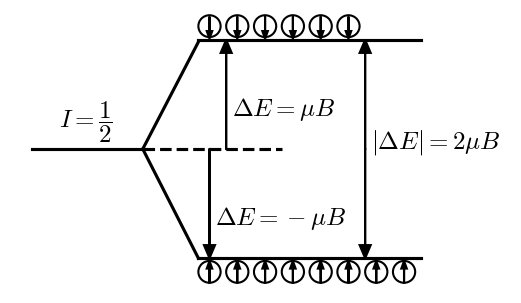
\includegraphics[width=.5\linewidth]{figures/Zeeman_effect.png}
    \caption{Zeeman splitting of a spin-$1/2$ nucleus in a magnetic field $B$. The energy difference $\Delta E$ between the two spin states is proportional to $B$.\YZ{TODO edit equation in the figure. }}
    \label{fig:Zeeman_effect}
\end{figure}

At thermal equilibrium, the spin populations obey the Boltzmann distribution.
In the high-temperature limit $\Delta E \ll k_B T$ (satisfied for all conditions in this thesis), the fractional spin polarization is
\begin{equation}
    p \approx \frac{\hbar \gamma B_0}{2 k_B T}
    \,.\label{eq:thermalp}
\end{equation}
At $B_0 = \SI{1}{\tesla}$ and $T = \SI{300}{\kelvin}$, the proton thermal polarization is only $p \approx \num{3e-6}$\,\cite{Zhang2026_Dissertation_ipynb_1_Introduction}.
Hyperpolarization techniques---such as spin-exchange optical pumping (SEOP) or parahydrogen-induced polarization (PHIP)---can boost $p$ by several orders of magnitud\,\cite{Eills2023_Spin_Hyperpolarization}. 
% , which is the main route to improved sensitivity identified in this thesis.


\subsection{Spin-projection noise}\label{sec:intro:NMR:SPN}
Even in the absence of a bias magnetic field, an ensemble of $N$ spins does not cancel perfectly to give a zero net magnetization. 
Statistical fluctuations leave a residual transverse moment of order $\sqrt{N}\,\mu$ (where $\mu = \hbar\gamma/2$ is the nuclear magneton), giving a magnetization noise floor
\begin{equation}
    M_\mathrm{SPN} \sim \frac{\sqrt{N}\,\mu}{V}
    \,.\label{eq:SPN}
\end{equation}
This spin-projection noise (SPN) is the fundamental quantum limit for spin measurements\,\cite{Bloch1946_NuclearInduction, Mitchell2020_MagSensors, Aybas_2021_Quantum_sensitivity}.
% In the ALP-search context it sets the minimum detectable magnetization\,\cite{Bloch1946_NuclearInduction, Mitchell2020_MagSensors, Aybas_2021_Quantum_sensitivity}. 
%  and is listed in Table~\ref{tab:parameters} for the experimental parameters of this work.
% how small this SPN can be?
For a sample of \SI{1}{\centi\meter\cubed} of liquid water, there are approximately $N \sim \num{1e23}$ protons. 
SPN gives a magnetization noise floor of $\sim \SI{4e-9}{\ampere/\meter}$. 
In comparison to the thermal-equilibrium magnetization of \SI{1e-8}{\ampere/\meter} at \SI{1}{\tesla} and \SI{300}{\kelvin}, the SPN is one order of magnitude less significant\,\cite{Zhang2026_Dissertation_ipynb_1_Introduction}.
In the scenario of less nuclear polarization or smaller sample volume, the SPN can become a limiting factor for the sensitivity of the experiment.

\subsection{Bloch equations}\label{sec:intro:bloch_eq}
The evolution of the nuclear spin magnetization $\mathbf{M}$ in the magnetic fields is governed by the Bloch equations\,\cite{Abragam1961_NuclearMagnetism}:
\begin{align}
    \frac{dM_x}{dt} &= \gamma\left(\mathbf{M}\times\mathbf{B}_\mathrm{eff}\right)_x - \frac{M_x}{T_2}\,,\label{eq:bloch_x}\\
    \frac{dM_y}{dt} &= \gamma\left(\mathbf{M}\times\mathbf{B}_\mathrm{eff}\right)_y - \frac{M_y}{T_2}\,,\label{eq:bloch_y}\\
    \frac{dM_z}{dt} &= \gamma\left(\mathbf{M}\times\mathbf{B}_\mathrm{eff}\right)_z - \frac{M_z-M_\mathrm{eqb}}{T_1}\,,\label{eq:bloch_z}
\end{align}
where $\mathbf{B}_\mathrm{eff}$ is the total effective field, $M_\mathrm{eqb}$ is the equilibrium magnetization, and $T_1$, $T_2$ are the longitudinal and transverse relaxation times.
In most NMR experiments, the bias field $\mathbf{B}_0$ is much larger than any other applied magnetic field. 
Therefore, the equations are most efficiently solved in the rotating coordinate frame (RCF), which removes the fast Larmor precession at $\nu_L$ in the laboratory frame and exposes the much slower dynamics induced by the additional fields.

% In the RCF, when the Larmor frequency is tuned to the ALP Compton frequency ($\nu_L = \nu_a$), the transverse component of $\mathbf{B}_a$ acts as a near-static drive.
% In the weak-drive limit ($\Omega_a T \ll 1$), the magnetization accumulates a small tipping angle $\xi$ and the transverse magnetization is $M_1 \approx M_\mathrm{eqb}\xi$.
% The ALP field is stochastic (Section~\ref{sec:theory:MWALP:stochasticity} and \ref{sec:theory:earthALP:coherence}), so $\xi$ and $M_1$ must be treated statistically; their rms\ values are derived in \YZ{add section reference for rms signal derivation}.

\subsection{Relaxations}\label{sec:intro:NMR:relaxation}

Relaxation describes the return of the spin ensemble toward equilibrium after it has been perturbed.
% relaxation time charaterizes how quickly the magnetization returns to equilibrium. 
In most of the NMR experiments, a bias magnetic field is applied, which defines the longitudinal direction, and the transverse plane is perpendicular to it\footnote{There are NMR experiments where a zero to ultra-low field (ZULF) is applied to study phenomena like the spin-spin interaction, which are difficult to observe at high fields. \YZ{add ref to zulf}}.


The return of the magnetization to equilibrium along the longitudinal direction is induced by energy exchange with the environment (spin-lattice relaxation) or through spin-spin interactions (spin-spin relaxation). 
Its speed is characterized by the relaxation time $T_1$ or relaxation rate $1/T_1$. 
The ``return'' can happen in two directions: when longitudinal magnetization is smaller than the equilibrium value, it grows toward the equilibrium; when it is larger (hyperpolarized), it decays. 
A short $T_1$ is helpful for rapid repetition of measurements using thermally polarized samples, while for hyperpolarized samples, a long $T_1$ is preferred to preserve polarization for longer measurements.
Its duration can be tuned by adjusting settings such as the bias field, temperature, and sample composition. 
For instance, oxygen is a paramagnetic molecule and dissolved oxygen in the sample can shorten $T_1$ by providing an additional relaxation channel. 

% \begin{figure}
%     \centering
%     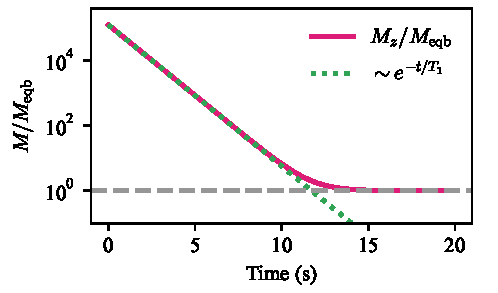
\includegraphics[width=.99\textwidth]{figures/T1_hyperpolarized.pdf}
%     \caption{Simulated $T_1$ relaxation of a hyperpolarized sample in a static bias field. The axial magnetization $M_z$ is normalized by the equilibrium magnetization $M_\mathrm{eqb}$.}
%     \label{fig:T1_hyperpolarized}
% \end{figure}
% As shown in Figure~\ref{fig:T1_hyperpolarized}, the hyperpolarized sample exhibits a long longitudinal relaxation time.


The transverse relaxation, determining how quickly coherent precession dephases, is characterized by several different time scales, including $T_2$, $T_\delta$ and $T_2^*$. 
$T_2$ characterizes microscopic spin-spin interactions and $T_\delta$ quantifies the dephasing caused by macroscopic magnetic-field inhomogeneity across the sample volume.
$T_2^*$ is the effective transverse relaxation time that incorporates both contributions, and it is always shorter than either of the two, as given by the relation
\begin{equation}
    \frac{1}{T_2^*} = \frac{1}{T_2} + \frac{1}{T_\delta}
    \,.\label{eq:T2star}
\end{equation}
The $T_2$ time can be adjusted by changing the sample composition, while $T_\delta$ can be prolonged by improving the field homogeneity through shimming. 

For brevity, the relaxations are referred to by the symbols of their characteristic time scales in this thesis, like $T_1$ relaxation.  

% TODO delete the follow part in comments
% For $T_1$ return of the magnetization to equilibrium
% longitudinal relaxation $T_1$ characterizes how quickly the magnetization along the bias magnetic field returns to equilibrium.  
% When the magnetization is smaller than the equilibrium value, the 

% Longitudinal relaxation governs how the population difference between spin states rebuilds after perturbation.

% Because field inhomogeneity can be reduced by shimming (Chapter~\ref{chap:experiment}), $T_2^*$ is experimentally controllable, but $T_2$ sets an intrinsic upper bound.


% Longer $T_2^*$ improves sensitivity in all four signal regimes derived in Chapter~\ref{chap:theory}.
% These time scales are central to the thesis because they set the window over which the ALP-induced signal can be observed coherently.

% Transverse relaxation combines microscopic spin-spin interactions ($T_2$) and macroscopic field inhomogeneity ($T_\delta$) as given in Equation~\eqref{eq:T2star}.
% It determines the free-decay signal and directly controls the linewidth in the frequency domain.
% For field searches, a narrower linewidth can improve sensitivity, but only if the coherence time remains long enough to integrate signal power efficiently.
% TODO write more about relaxation?
% \subsubsection{$T_1$ relaxation}\label{sec:intro:NMR:relaxation:T1}

% For sample initially polarized by the bias field

% \subsubsection{$T_2^*$ relaxation}\label{sec:intro:NMR:relaxation:T2}

% \subsubsection{Cross relaxation}
% For samples containing multiple spin species, cross relaxation can transfer energy between the different species.
% Cross relaxation transfers energy between coupled spin species or spin reservoirs.
% In samples containing more than one spin system, it modifies the effective relaxation rates of each species.


% \subsection{Chemical shift}
% Chemical shielding modifies the local field at a nucleus and shifts its resonance frequency.
% The shift is small in absolute terms but distinguishes nuclei in different chemical environments.

% In this thesis, chemical shift contributes to the spectral structure of the sample and offsets the resonance from the bare Larmor value.

% \subsection{Spin-spin coupling}
% Coupling between nuclear spins splits resonance lines into multiplets.
% The resulting J-coupling pattern provides a spectral fingerprint for molecular identification, which helps distinguish genuine NMR signals from noise.

% For the calibration sample, J-coupling produces a resolved multiplet that serves as a reliable spectral reference.

\subsection{Experimental schemes}
% Two pulse-based schemes are especially useful.
In a common NMR experiment, the sample is first thermally polarized in a bias field, then perturbed by excitation pulses to generate precession signal in the transverse plane, and finally allowed to relax back to equilibrium.
The excitation pulses tip the magnetization away from the longitudinal axis. The tipping angle is determined by the pulse duration and amplitude
\begin{equation}
    \theta = \gamma B_\mathrm{exc} t
    \,.\label{eq:tipping_angle}
\end{equation}
where $\theta$ is the tipping angle, $B_\mathrm{exc}$ is the amplitude of the excitation field, and $t$ is the pulse duration.
The tipping angle is typically $\pi/2$ or $\pi$. 
These are also referred to as $\SI{90}{\degree}$ and $\SI{180}{\degree}$ pulses in the NMR literature.


% Both are diagnostic tools that help characterize the apparatus before an axion measurement.

\subsubsection{Free decay}\label{sec:intro:NMR:scheme:1Pulse}
After a $\pi/2$ pulse, the magnetization is tipped into the transverse plane and then decays with the relaxation time $T_2^*$. 
The resulting free decay signal, following an exponential decay envelope ($\exp(-t/T_2^*)$), is an observable for measuring the $T_2^*$ and the Larmor frequency.
The process is illustrated in Figure~\ref{fig:PulsedNMR_Schematic}.
\begin{figure}
    \centering
    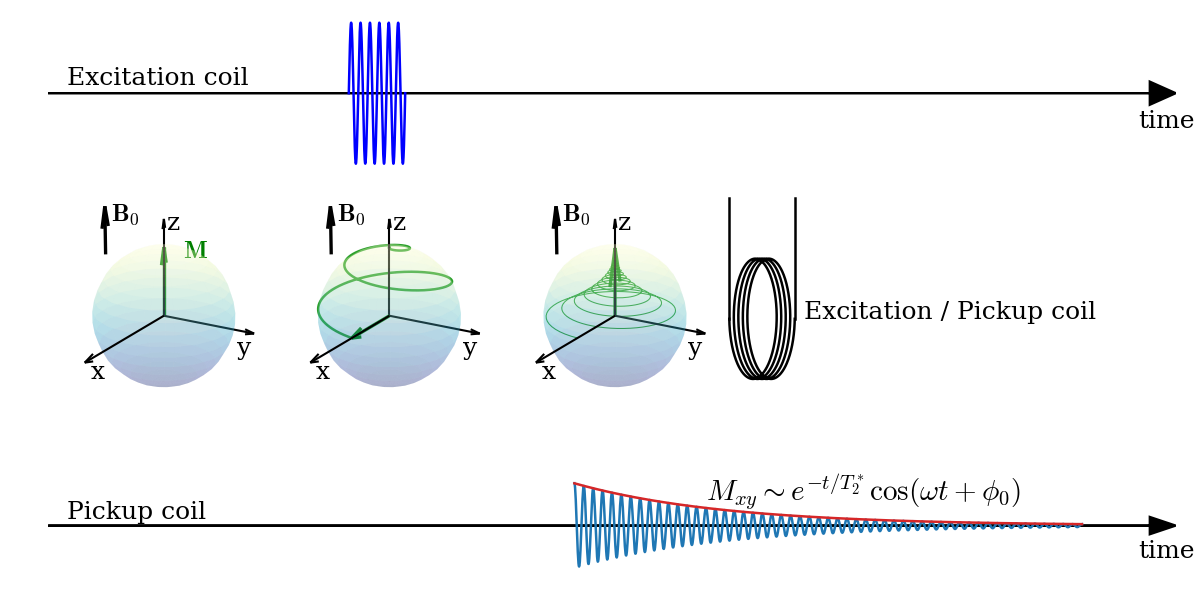
\includegraphics[width=.99\textwidth]{figures/PulsedNMR_Schematic_20220911.png}
    \caption{Schematic of pulsed NMR sequences in the laboratory frame.}
    \label{fig:PulsedNMR_Schematic}
\end{figure}

If the measurable is the induction in a pickup coil generated by spin precession, the signal is called free-induction decay (FID). 
However, in this thesis, it is the magnetic flux, instead of the induction, that is measured.
Therefore, the term ``free decay'' is used for inconclusiveness. 


\subsubsection{Spin echo and CPMG sequence}\label{sec:intro:NMR:scheme:echo}

$T_2^*$ relaxation leads to dephasing of the transverse magnetization due to differences in the Larmor frequency across the sample volume.
If a $\pi$ pulse is applied after a $\pi/2$ pulse, the magnetization is flipped by \SI{180}{\degree}, and the dephasing is reversed. 
The reversed dephasing, or ``refocusing,'' produces a spin echo, as illustrated in Figure~\ref{fig:SpinEcho_Schematic}.
% Spin echo uses a $\pi$ pulse after a $\pi/2$ pulse to reverse dephasing due to field inhomogeneity. 
This spin-echo scheme separates spin-spin relaxation from relaxation caused by field inhomogeneity.\YZ{add reference for spin echo and cpmg}

\begin{figure}
    \centering
    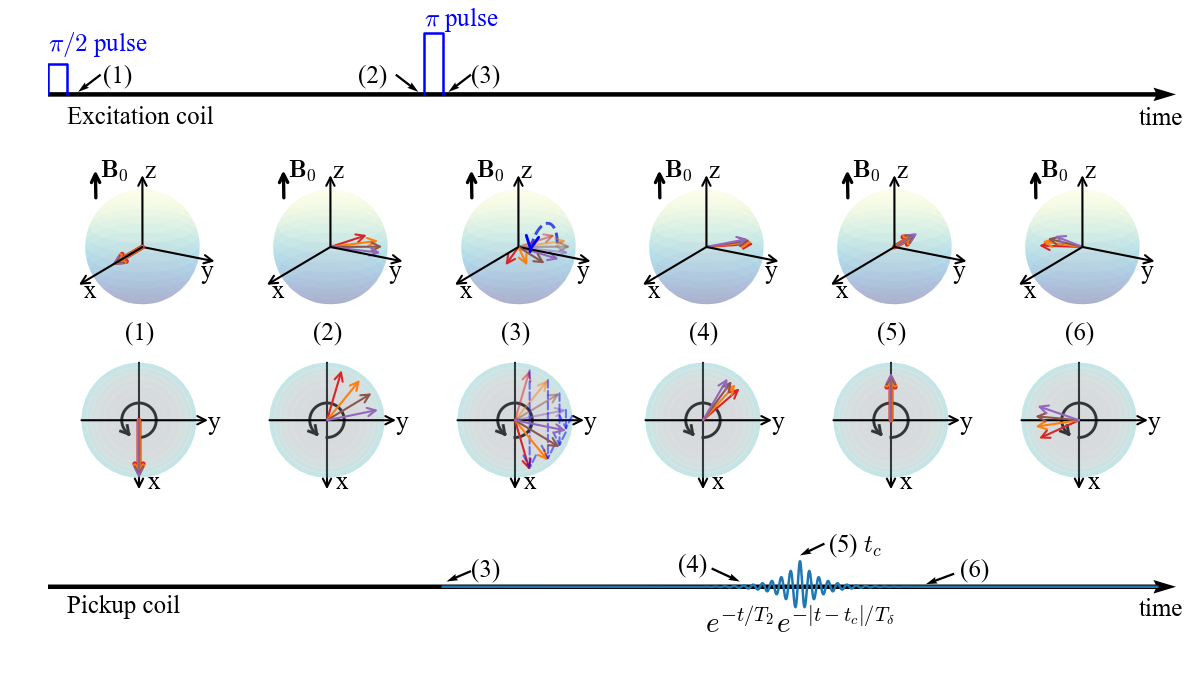
\includegraphics[width=.99\textwidth]{figures/SpinEcho_Schematic_20220918.png}
    \caption{Schematic of the spin-echo sequence in the laboratory frame. The $\pi$ pulse reverses dephasing from static field inhomogeneity, producing an echo at time $2\tau$. \YZ{modify the pic} }
    \label{fig:SpinEcho_Schematic}
\end{figure}

% \subsubsection{CPMG sequence}\label{sec:intro:NMR:scheme:CPMG}
The Carr--Purcell--Meiboom--Gill (CPMG) sequence extends the spin-echo scheme by applying a $\pi/2$ pulse followed by a train of $\pi$ refocusing pulses.
Each refocusing pulse produces an echo, and the decay of the echo amplitudes gives a measurement of $T_2$.
In this thesis, CPMG is used as a pulsed-NMR diagnostic to characterize the sample relaxation before and after measurements.


\section{Dark matter hypothesis}\label{sec:intro:DM}

The prevailing cosmological framework is the $\Lambda$ cold-dark-matter ($\Lambda$CDM) model.
It combines a cosmological constant $\Lambda$, which describes the accelerated expansion of the universe, with a cold, nonrelativistic, and collisionless dark-matter component.
$\Lambda$CDM provides a successful common description of the cosmic microwave background, the growth of large-scale structure, galaxy clustering, and the expansion history.
Its success establishes a powerful baseline, but it does not identify the physical nature of dark matter, and its assumptions are being challenged on galactic and subgalactic scales.

An alternative to dark matter is modified gravity, most prominently Modified Newtonian Dynamics (MOND), which replaces Newtonian dynamics at very small accelerations rather than introducing unseen matter.
MOND was originally proposed to explain flat galaxy rotation curves and can reproduce several galactic-scale regularities with an acceleration scale $a_0 \sim 10^{-10}\,\mathrm{m\,s^{-2}}$\,\cite{Milgrom1983_MOND,Banik2022_MONDreview,Zhao2005_MONDglobularClusters}. 
MOND captures several galactic-scale regularities, but it faces difficulties in explaining galaxy clusters and cosmological data. 
This thesis aims to test the dark-matter hypothesis, so it does not focus on modified-gravity alternatives. 


\subsection{Astronomical evidence}

The concept of dark matter arose from astronomical observations that could not be explained by visible matter and standard gravity alone.
Here ``visible'' refers to baryonic matter that emits or scatters electromagnetic radiation, while ``dark'' refers to matter that interacts primarily through gravity.
Galaxy rotation curves provide a classic example: orbital speeds remain approximately constant far beyond the bright stellar disk, rather than decreasing as expected if most of the mass followed the visible matter\,\cite{rubin1970rotation,Sofue_Rubin_2001_RotationCurves}.
This behavior indicates that galaxies are embedded in extended, non-luminous mass halos.

Evidence at larger scales comes from gravitational lensing and colliding galaxy clusters.
In the Bullet Cluster, the dominant gravitational mass inferred from lensing is spatially separated from the baryonic mass which is mostly hot X-ray-emitting gas\,\cite{Clowe_2006_DirectEmpiricalProof}.
This separation is naturally explained if most of the mass is dark and collisionless during the cluster collision, and disfavors the MOND theory.
Independently, the cosmic microwave background, big-bang nucleosynthesis, and the growth of large-scale structure require substantially more gravitating matter than can be supplied by baryons.
Cosmological fits assign roughly \SI{5}{\%} of the cosmic energy budget to baryonic matter and about \SI{27}{\%} to dark matter\,\cite{ade2016planck}.


\subsection{Recent developments}

Despite the large-scale success of $\Lambda$CDM, its simplest collisionless cold-dark-matter realization faces open questions on smaller scales.
Simulations and observations can differ in the predicted abundance of dwarf satellites and in the inner density profiles and diversity of low-mass halos.
These tensions may reflect incompletely modeled baryonic processes, or they may indicate that the dark-matter sector is warmer, wave-like, or self-interacting rather than perfectly cold and collisionless\,\cite{Vegetti2026_ChallengeCDMWDM}.

Recent observations increasingly test these possibilities.
Work involving Roberto Abraham and collaborators identified the ultra-diffuse galaxy NGC~1052--DF2 as having an unusually small dark-matter content\,\cite{vanDokkum2018_DarkMatterDeficient}, referred to as ``dark matter deficiency''.
Follow-up work proposed that this galaxy and related objects form a trail produced by a high-speed ``bullet-dwarf'' collision that separated stars and gas from their original dark-matter halos\,\cite{vanDokkum2022_BulletDwarfTrail}.
Such systems probe the normally tight connection between galaxies and their halos and may help clarify how baryonic and dark matter can become spatially separated.
They challenge simple galaxy--halo relations, although collision-driven formation scenarios may accommodate them within the broader $\Lambda$CDM framework.

The central structures of halos provide a more direct test of the collisionless-CDM assumption.
In self-interacting dark matter (SIDM) models, scattering between dark-matter particles redistributes energy and changes the central density profiles of halos.
A recent strong-lensing analysis led by Simona Vegetti found an unusually compact perturber whose inferred structure, if dark-matter dominated, is difficult to reconcile with conventional cold or warm dark matter\,\cite{Powell2025_MillionSolarMassObject}.
One possible interpretation is an SIDM halo that underwent gravothermal core collapse and formed a central black hole\,\cite{Vegetti2026_ChallengeCDMWDM}.
This interpretation is not yet unique, but it highlights the challenges at $\Lambda$CDM at small scales.


\subsection{Dark matter models}

The observations establish the gravitational role of dark matter but do not identify its microscopic nature.
In this sense, $\Lambda$CDM specifies the required large-scale behavior of the dominant matter component rather than a unique particle.
Proposed realizations cover an enormous range of mass and behavior, and several alternatives modify the small-scale predictions of minimal cold dark matter.
At the low-mass end, fuzzy dark matter consists of bosons with masses $\sim\SI{e-22}{\eV/c^2}$; their kiloparsec-scale de~Broglie wavelengths make wave effects relevant to galactic structure\,\cite{Lam2017_PhysRevD}.
Other particle candidates include sterile neutrinos, warm dark matter (WDM), weakly interacting massive particles (WIMPs), and self-interacting particles.
At the opposite, macroscopic end, primordial black holes (PBHs) formed in the early universe could contribute some or all of the dark matter within the remaining observationally allowed mass windows\,\cite{Carr2020_PBH_DarkMatter}.
Laboratory searches consequently range from particle-collision and scattering experiments to gravitational surveys and precision measurements\,\cite{Kimball2023_search}.

Among all these dark matter models, axions and axionlike particles occupy a particularly interesting part of this landscape.
Their low masses permit a coherent, wave-like dark-matter field, while their weak non-gravitational couplings make laboratory searches possible.
The following section introduces their origin, field properties, and coupling to nuclear spins.

\section{Axions and axionlike particles}\label{sec:intro:axions}
\subsection{Axion}

Why quantum chromodynamics (QCD) appears to conserve $CP$ ($C$ and $P$ are the charge conjugation and parity operators, respectively) so precisely even though the theory allows a $CP$-violating term that should otherwise be observable? 
This is the strong $CP$ problem. 
In 1977, Peccei and Quinn proposed axion as a solution to the strong $CP$ problem
In 1977, Peccei and Quinn proposed a solution to the strong $CP$ problem by introducing a new global $U(1)$ symmetry, now called the Peccei--Quinn symmetry\,\cite{PecceiQuinn1977_CPConservation_PRL,PecceiQuinn1977_ConstraintsCP_PRD}. 
The symmetry is spontaneously broken at a high energy scale $f_a$, which generates a pseudo-Goldstone boson called the axion.
The potential of the axion field is minimized at the $CP$-conserving point, naturally explaining why the strong interaction conserves $CP$. 
% The symmetry breaking at the scale $f_a$ generates a pseudo-Goldstone boson called axion whose potential is minimized at the $CP$-conserving point, naturally explaining why the strong interaction conserves $CP$.
The axion acquires a mass $m_a \sim \Lambda_\mathrm{QCD}^2/f_a$ from QCD dynamics.
To distinguish this axion model from other axionlike particles, it is also referred to as the ``QCD axion'' or ``PQ-axion'' in literatures.
% The QCD axion is a hypothetical pseudoscalar particle that appears when a global symmetry is introduced to explain why strong interactions conserve $CP$ so well.
% Its properties are tightly linked to the QCD scale, which makes it a special case rather than the most general one.
Cosmological production via the misalignment mechanism constrains $f_a \lesssim 10^{12}$ GeV (axion mass $\gtrsim \SI{6}{\micro\electronvolt}$) if the axion is to constitute all dark matter\,\cite{diCortona2016_QCDAxionPrecisely}.
% TODO remove all comments in the second proofreading

\subsection{Axionlike particles}\label{sec:intro:ALP}

Axionlike-particles (ALPs) emerge when a global symmetry is broken\,\cite{Weinberg1978_NewLightBoson,Wilczek1978_StrongPTInvariance, Kim1979_WeakInteractionSinglet, Shifman1980_ConfinementCP, Dine1981_HarmlessAxion, Zhitnitsky1980_WeinbergCP}.
ALPs share the oscillatory and weakly coupled character of the QCD axion, but their mass range can be much wider, since the mechanism of ALP production is different from QCD axion.
There have been investigations in determining the ALP mass range from astronomical observations\,\cite{Marsh2016_AxionCosmology} and theoretical studies\,\cite{Zhitnitsky1980_WeinbergCP}.
However, in this thesis, the ALP mass is regarded as a free parameter, and the search is performed in a range which the experiment is sensitive to.

\subsubsection{Wave nature}

A nonrelativistic ALP with mass $m_a$ and velocity $\mathbf{v}_a$ ($v_a \ll c$) has energy $E_a \simeq m_a c^2+\tfrac{1}{2}m_a v_a^2$, and Compton frequency $\nu_a=E_a/h$, where $h$ is Planck's constant and $c$ is the speed of light in vacuum.
Its de~Broglie wavelength is
\begin{equation}
    \lambda_{\mathrm{dB}}=\frac{h}{m_a v_a}
    \,.\label{eq:lambda_dB}
\end{equation}
For an ultralight ALP this wavelength can be macroscopic ($\gtrsim \SI{100}{\micro\meter}$). 
Assuming axionlike dark matter is cold, its velocity is expected to be smaller than the escape velocity of the Milky Way halo $v_\mathrm{esc} = \SI{550}{\km/\s}$\,\cite{Evans2019_SHMRefined}.
The minimum de~Broglie wavelength is $\lambda_{\mathrm{dB}} \sim \SI{7e-5}{\meter}$ for ALPs in the Milky Way ($m_a \leq \SI{10}{\eV/c^2}$)\,\cite{Zhang2026_Dissertation_ipynb_1_Introduction}.
For the ALP mass range relevant to this thesis ($m_a \leq \SI{2.5}{\micro\electronvolt}$), the de~Broglie wavelength $\lambda_{\mathrm{dB}} \geq \SI{270}{\meter}$, much larger than the size of the laboratory.
Therefore, the amplitude of the ALP field can be approximated as uniform over the laboratory. 

The ALP field of a single free ALP mode can be written as a real field: 
\begin{align}
     a(\mathbf{r},t)
     &=\sqrt{\frac{\hbar^3c}{2 m_a}}\,
      \left(\Psi(\mathbf{r},t) + \Psi^*(\mathbf{r},t)\right)\\
    &=\sqrt{\frac{\hbar^3c}{m_a}}\,
      \Re\left[\Psi(\mathbf{r},t)\right]
    \,,\label{eq:ALP_single_wavefunction}
\end{align}
where $\Psi$ is wavefunction of a single ALP. 
Consider an ensemble of $N_a$ ALPs with local energy density $\rho_a$.
Its number density is
\begin{equation}
    n_a=\frac{\rho_a}{m_a c^2}
    \,,\label{eq:na}
\end{equation}
and the mean occupation number within a de~Broglie volume is approximately
\begin{equation}
    N_a\simeq n_a\lambda_{\mathrm{dB}}^3
    =\frac{\rho_a h^3}{m_a^4 v_a^3 c^2}
    \,.\label{eq:occupation}
\end{equation}
If the ALP is the dominant dark-matter component, $\rho_a$ is close to the local dark-matter energy density $\rho_\mathrm{DM} \sim \SI{0.4}{\GeV/\cm^3}$\,\cite{Evans2019_SHMRefined}. 
Considering ALP mass relevant to this thesis $m_a \leq \SI{2.5}{\micro\electronvolt}$ and velocity $v_a \leq v_\mathrm{esc} = \SI{550}{\km/\s}$, the occupation number is $N_a \geq \SI{3e27}{}$, much larger than unity\,\cite{Zhang2026_Dissertation_ipynb_1_Introduction}.
Therefore, what is measured in the experiment is the collective effect of many ALPs instead of rare single-particle events. 
% The highly occupied quantum field can therefore be approximated by a classical field. \YZ{really?}
% The ensemble is coherent over a length scale set by the de~Broglie wavelength.
% Its phase and spatial structure can be described by a complex wavefunction $\Psi(\mathbf{r},t)$, which may contain one or more occupied modes.

For $N_a$ ALPs that are collectively described by a wavefunction normalized as $\int|\Psi|^2\,d^3r=1$, the associated scalar field is the appropriately scaled real part of the wavefunction like in Equation~\eqref{eq:ALP_single_wavefunction}:
\begin{equation}
    a(\mathbf{r},t)
    =\sqrt{\frac{2N_a\hbar^3c}{m_a}}\,
      \Re\left[\Psi(\mathbf{r},t)\right]
    \,.\label{eq:a0_Psi_real}
\end{equation}
The local, time-averaged energy density is $\rho_a=m_a c^2N_a\langle|\Psi(\mathbf{r},t)|^2\rangle_t$, where $\langle|\Psi(\mathbf{r},t)|^2\rangle_t$ denotes the time average.
Eliminating $N_a$ gives
\begin{align}
    a(\mathbf{r},t)
    &=\sqrt{\frac{2\hbar^3\rho_a}{m_a^2c}}\,
      \frac{\Re\left[\Psi(\mathbf{r},t)\right]}
      {\langle|\Psi(\mathbf{r},t)|^2\rangle_t^{1/2}}
      \notag\\
    &=a_0\,
      \frac{\Re\left[\Psi(\mathbf{r},t)\right]}
      {\langle|\Psi(\mathbf{r},t)|^2\rangle_t^{1/2}}
    \,,\label{eq:a0_rhoDM_Psi_real}
\end{align}
where 
\begin{equation}
    a_0
    =\sqrt{\frac{2\rho_a\hbar^3}{m_a^2c}}
    \,.\label{eq:a0_rhoDM}
\end{equation}
is the local field amplitude.  
% For the approximately homogeneous Milky Way field, $\rho_a$ is replaced by the local halo density $\rho_{DM}$. 
% For an Earth-bound state, its spatial dependence is determined by the bound-state wavefunction.
% \subsubsection{Coherent and stochastic fields}
If all $N_a$ ALPs occupy the same mode, the corresponding local field takes the plane-wave form
\begin{equation}
    a(\mathbf{r},t)
    =a_0\cos\left(2\pi\nu_a t-\mathbf{k}\cdot\mathbf{r}+\phi\right)
    \,,\label{eq:ALP_field}
\end{equation}
over a region where the axion density can be treated as uniform. 
A realistic ALP wavefunction generally contains many modes and may be written as
\begin{equation}
    \Psi(\mathbf{r},t)
    =\sum_j C_j
    \exp\left[-i\left(2\pi\nu_jt-\mathbf{k}_j\cdot\mathbf{r}+\phi_j\right)\right]
    \,.\label{eq:ALP_sum}
\end{equation}
The coefficients $C_j$ encode the populations of the modes and are fixed by the normalization of $\Psi$.
The physical scalar field remains proportional to $\Re[\Psi]$ according to Equation~\eqref{eq:a0_rhoDM_Psi_real}.
Moreover, if ALPs occupy many modes, the resulting field is a superposition of those modes. 
% Because the modes have different velocities, they also have slightly different frequencies.
% Their relative phases consequently drift: over short times the sum resembles a coherent oscillation, whereas over longer times its effective amplitude and phase fluctuate. 
The interference of many modes with different velocities makes the field stochastic. 
The stochasticity is characterized by the coherence time. 
Chapter~\ref{chap:theory} develops this behavior for Milky Way axion halo and Earth-bound axion halo.

\subsection{Non-gravitational interactions}
An oscillating ALP field can potentially produce three non-gravitational interactions: it may couple to photons, generating an electromagnetic field; its coupling to gluons induces oscillating $CP$-odd nuclear moments such as a nuclear electric dipole moment (EDM); its gradient coupling to nucleons and electrons acts as oscillating magnetic fields on nuclear and electron spins. \,\cite{GrahamNewobservables}.
All three effects oscillate at a frequency set primarily by the ALP mass and can therefore be sought with resonant precision measurements.

This thesis focuses on the gradient coupling to nucleons, also known as the ``axion-wind'' coupling.
The nucleon Hamiltonian in the presence of an ALP field background can be written as
\begin{equation}
    H_{\mathrm{aNN}} = c g_{\mathrm{aNN}}\,{\boldsymbol\nabla}a\cdot\mathbf{I}
    \,,\label{eq:HaNN}
\end{equation}
where $g_{\mathrm{aNN}}$ is the coupling strength in $\SI{}{\GeV^{-1}}$ and $\mathbf{I}$ is the nuclear spin operator. 
% For spin-$1/2$ nuclei, $\mathbf{I} = \hbar {\boldsymbol\sigma_n}/2$, where ${\boldsymbol\sigma_n}$ is the dimensionless Pauli spin operator.
In this form of Hamiltonian, $g_{\mathrm{aNN}} a_0$ becomes dimensionless. 
The amplitude $a_0$ is fixed by the local dark-matter density through Equation~\eqref{eq:a0_rhoDM} and has dimensions of energy. 
In some papers, nuclear spin operator $\mathbf{I}$ is substituted with $\hbar {\boldsymbol\sigma_n}/2$, where $ {\boldsymbol\sigma_n}$, where ${\boldsymbol\sigma_n}$ is the dimensionless Pauli spin operator.

% \YZ{remove this paragraph? }
% Expanded:
% \begin{equation}
%     H_{\mathrm{aNN}} = c g_{\mathrm{aNN}} a_0
%     \sin(2\pi\nu_a t - \mathbf{k}\cdot\mathbf{r} + \phi)
%     m_a \,\mathbf{v}_a\cdot\mathbf{I}/ \hbar
%     \,,\label{eq:HaNN_vel}
% \end{equation}

% TODO move the following to the theory chapter
Comparing this with the NMR Hamiltonian $H_\mathrm{NMR} = -\gamma\mathbf{B}\cdot\mathbf{I}$, the ALP gradient acts as an effective oscillating pseudomagnetic field, where the Rabi frequency and field amplitude are given by
\begin{equation}
    \Omega_a(t) = c g_{\mathrm{aNN}}\,{\boldsymbol\nabla}a
    \,\label{eq:Omega_a}
\end{equation}
and
\begin{equation}
    \mathbf{B}_a(t) = \frac{c g_{\mathrm{aNN}}\,{\boldsymbol\nabla}a}{\gamma}
    \,.\label{eq:Bpseudo}
\end{equation}
This gradient coupling oscillates at the ALP Compton frequency and can drive resonant spin precession when the Larmor frequency matches $\nu_a$. 
% The search for this coupling is the subject of Chapter~\ref{chap:results}.
% \YZ{add some examples to show equivalent Ba field magnitude?}


% The rms Rabi frequency of the pseudomagnetic field can be found by the Hamiltonian in Equation~\eqref{eq:HaNN}\,\cite{Centers2021Stochastic,Yuzhe2023_FrequencyScanning}
% % \begin{equation}
% %     \Omega_a = \dfrac{1}{2}\, g_{\mathrm{aNN}} \sqrt{2\hbar c\, \rho_{DM}}\, v_{\bot}
% %     \,,\label{eq:Omega_a}
% % \end{equation}
% \begin{equation}
%     \Omega_a = \dfrac{1}{2\hbar} c g_\mathrm{aNN} a_0 m_a v_{\bot} = \dfrac{1}{2} g_{\mathrm{aNN}} \sqrt{2\hbar c \rho_{DM}} v_{\bot}
%     \,,\label{eq:Omega_a_MW}
% \end{equation}
% where $v_{\bot}$ is the component of the ALP-detector relative velocity perpendicular to $\mathbf{B}_0$.
% Taking $v_{\bot} = \SI{220}{\km\per\second}$, we have $\Omega_a/2\pi = g_{\mathrm{aNN}} \times \SI{0.2}{\GeV\cdot\Hz}$.
% For $g_{\mathrm{aNN}} \lesssim 10^{-10}\,\SI{}{\GeV^{-1}}$, the Rabi period $2\pi/\Omega_a \gtrsim 1000\,\mathrm{yr}$, confirming that the ALP field is a weak drive on the spins.
% \YZ{What about that factor of one half?
% Check the values!
% Mention the weak-drive limit.}



\section{CASPEr project}\label{sec:intro:CASPEr}

\subsection{ALP search with spin haloscope}

Depending on the theoretical model, different schemes of sexperiments are adopted to search for ALP-induced spin precession\,\cite{Kimball2023_search}. 
Such experiments are often referred to as spin haloscopes. 
For example, the Global Network of Optical Magnetometers for Exotic physics searches (GNOME)\,\cite{Pustelny_AdP_GNOMEnovel, Pospelov_PhysRevLett_DomainWalls, Kimball_2018_PhysRevD_terrestrial, Masia-Roig_2020_Analysismethod, Afach_2021_topological} investigates transient exotic spin couplings. 
Other examples are Noble and Alkali Spin Detectors for Ultralight Coherent darK matter (NASDUCK) using Floquet NMR quantum detector\,\cite{bloch2105nasduck} and QUaerere AXions (QUAX) experiment probing the possible ALP-electron spin interaction\,\cite{Crescini2020_Ferromagnetic}. 

Cosmic Axion Spin Precession Experiment (CASPEr) is a project proposed in 2014\,\cite{CASPErProposal2014} that uses nuclear spins to search for ALP-induced spin precession.
The project has several branches, including ALP-gluon and ALP-fermion (ALP gradient) searches, and both low-magnetic-field and high-magnetic-field implementations.
% \subsection{The idea}
The central idea is to tune the NMR resonance to a frequency that matches the ALP Compton frequency.
If the two frequencies align, the ALP field applies a torque on the magnetization and induces a transverse magnetization in the sample.
Since the ALP mass is unknown, the search is performed through a frequency scan: either the signal appears at a particular resonance or the absence of a signal constrains the coupling strength over the scanned band.

\subsection{CASPEr-Electric and CASPEr-Comagnetometer}

CASPEr-Electric (CASPEr-E) searches for an oscillating nuclear EDM induced by the ALP-gluon coupling.
This moment generates an effective oscillating field along the nuclear spin axis in the presence of an electric field, enabling detection through NMR at the corresponding Compton frequency.

% \subsection{}
Comagnetometer configurations use two nuclear spin species in the same volume to suppress common-mode magnetic noise. 
The differential signal between the two species enhances sensitivity to a pseudomagnetic ALP field while rejecting electromagnetic backgrounds.
Early results were obtained with a liquid-state comagnetometer\,\cite{PhysRevLett.122.191302} and an ultralow-magnetic-field configuration\,\cite{CASPEr_ZULF_2019}.

\subsection{CASPEr-Gradient}\label{sec:intro:CASPEr:gradient}
CASPEr-Gradient searches for the ALP-fermion gradient coupling described by Equation~\eqref{eq:HaNN}.
Two setups in Mainz, Germany cover different ALP-mass ranges.
The CASPEr-Gradient-Lowfield experiment uses bias fields up to \SI{0.1}{\tesla}, corresponding to Larmor frequencies up to \SI{4.3}{\MHz}.
The CASPEr-Gradient-Highfield experiment uses a 0-to-\SI{14.1}{\tesla} magnet to reach frequencies up to \SI{600}{\MHz}.

A conceptual diagram of the lowfield apparatus is shown in Figure~\ref{fig:CASPEr_Apparatus}.
The cryostat contains a liquid helium reservoir, excitation and pickup coils, and a SQUID magnetometer.
A superconducting magnet produces the bias field $\mathbf{B}_0$, which sets the Larmor frequency and can be varied to scan ALP masses.

% resonance and broadband scheme
The resonance scheme is the main search strategy for CASPEr-Gradient-Lowfield.
The bias field is stepped through a range of values, and the NMR response is recorded at each step while no excitation is applied.
A resonant signal appears as a peak in the transverse magnetization when $\nu_L$ matches $\nu_a$.

The broadband scheme, on the other hand, continuously excites the NMR resonance without changing the bias field, looking for signals that are modulated by the ALP field. 

\begin{figure}[htb]
    \centering
    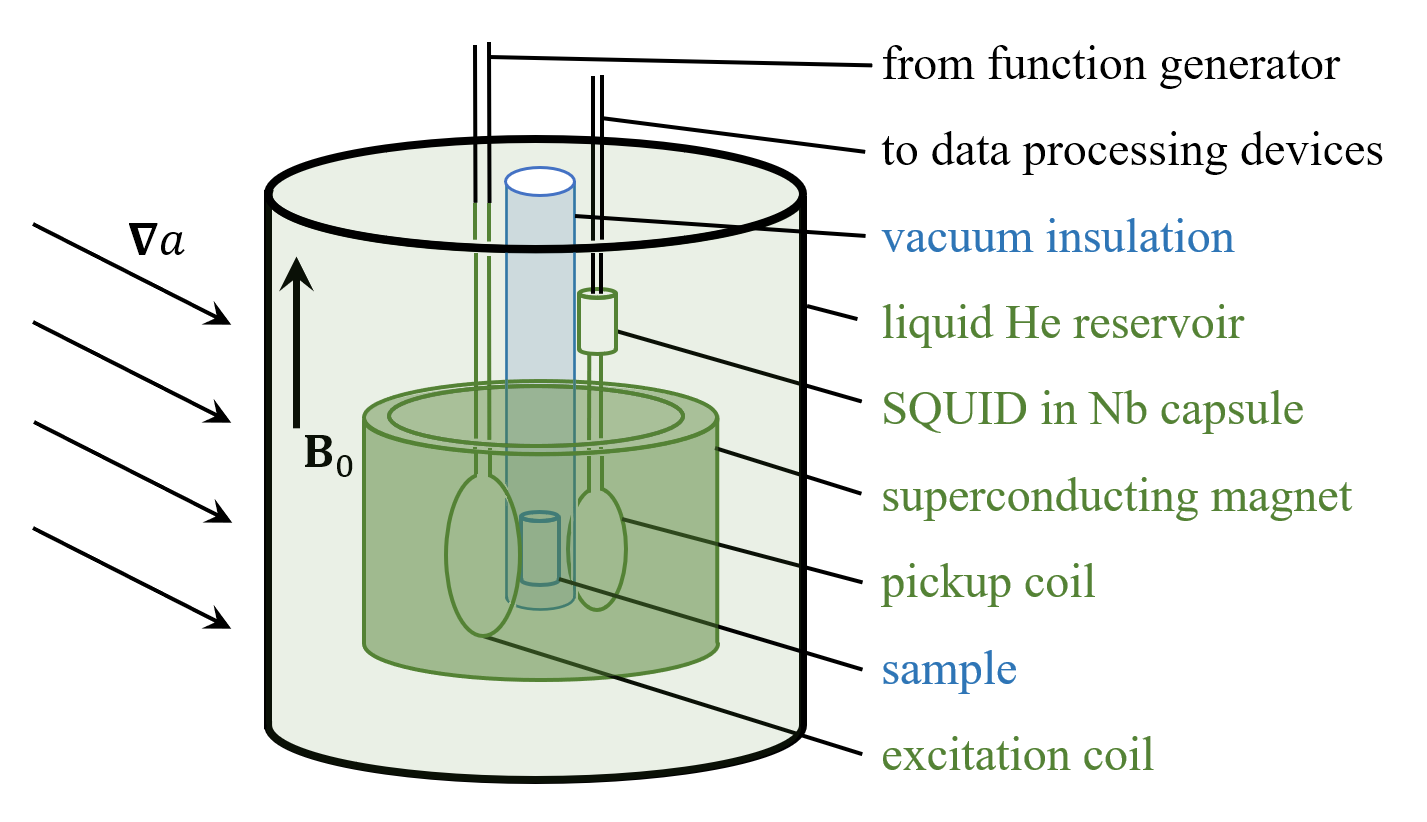
\includegraphics[width=0.65\linewidth]{figures/CASPEr_Apparatus_20230508.png}
    \caption{Conceptual diagram of the CASPEr-Gradient-Lowfield setup.
    Superconducting devices (dark green) are submerged in a liquid helium bath (light green).
    The excitation and pickup coils characterize the sample and detect the spin-precession signal.
    The sample temperature can be controlled independently of the helium bath, enabling measurements with both thermal and hyperpolarized samples.
    Reproduced from Ref.\,\cite{Yuzhe2023_FrequencyScanning} with permission.}
    \label{fig:CASPEr_Apparatus}
\end{figure}

Beyond ALP-fermion coupling, CASPEr-Gradient, as a sensitive magnetometer experiment, has the potential to search for other exotic physics, such as the axion-photon coupling and dark photon\,\cite{BerlinKahn2025_NewTechAxionDarkPhoton}.
Such potential is to be discussed in future works. 

\subsection{Candidate, exclusion, and sensitivity}

There are several unknown parameters in the ALP search, including the ALP mass, the coupling strengths, and the ratio of ALP density to the local dark-matter density.
In this thesis, it is assumed that ALPs constitute all of the local dark matter, and ALP mass and coupling strengths are treated as free parameters. 
These two parameters define the mass-coupling parameter space. 

Every haloscope is sensitive to a certain range of ALP masses. 
The ultimate goal for a haloscope is to detect the ALP at a particular mass and coupling strength in this parameter space. 
If no ALP \textbf{candidate} is found, the search sets \textbf{exclusion} on the ALP coupling strength over the searched mass range. 
People use ``limit'' and ``constraint'' interchangeably with ``exclusion'' in literatures, which have the same meaning.
If any candidate is found, no exclusion can be set below the coupling strength at that mass. 
The common practice is to leave gaps or openings in the exclusion to indicate the presence of candidates.

Besides exclusion, a haloscope can also report its \textbf{sensitivity} in the mass-coupling parameter space. 
The sensitivity in the parameter space is determined by the mass range that the haloscope can cover and the coupling strength that can be detected at each mass. 
Even before any search is performed, the \textbf{projected sensitivity} can be calculated based on the experimental parameters and the expected ALP signal. 

Figure~\ref{fig:AxionProton_with_Projections}, as an example of parameter space searched by haloscopes, summarizes the current status of the ALP-proton mass-coupling parameter space.

\begin{figure}
    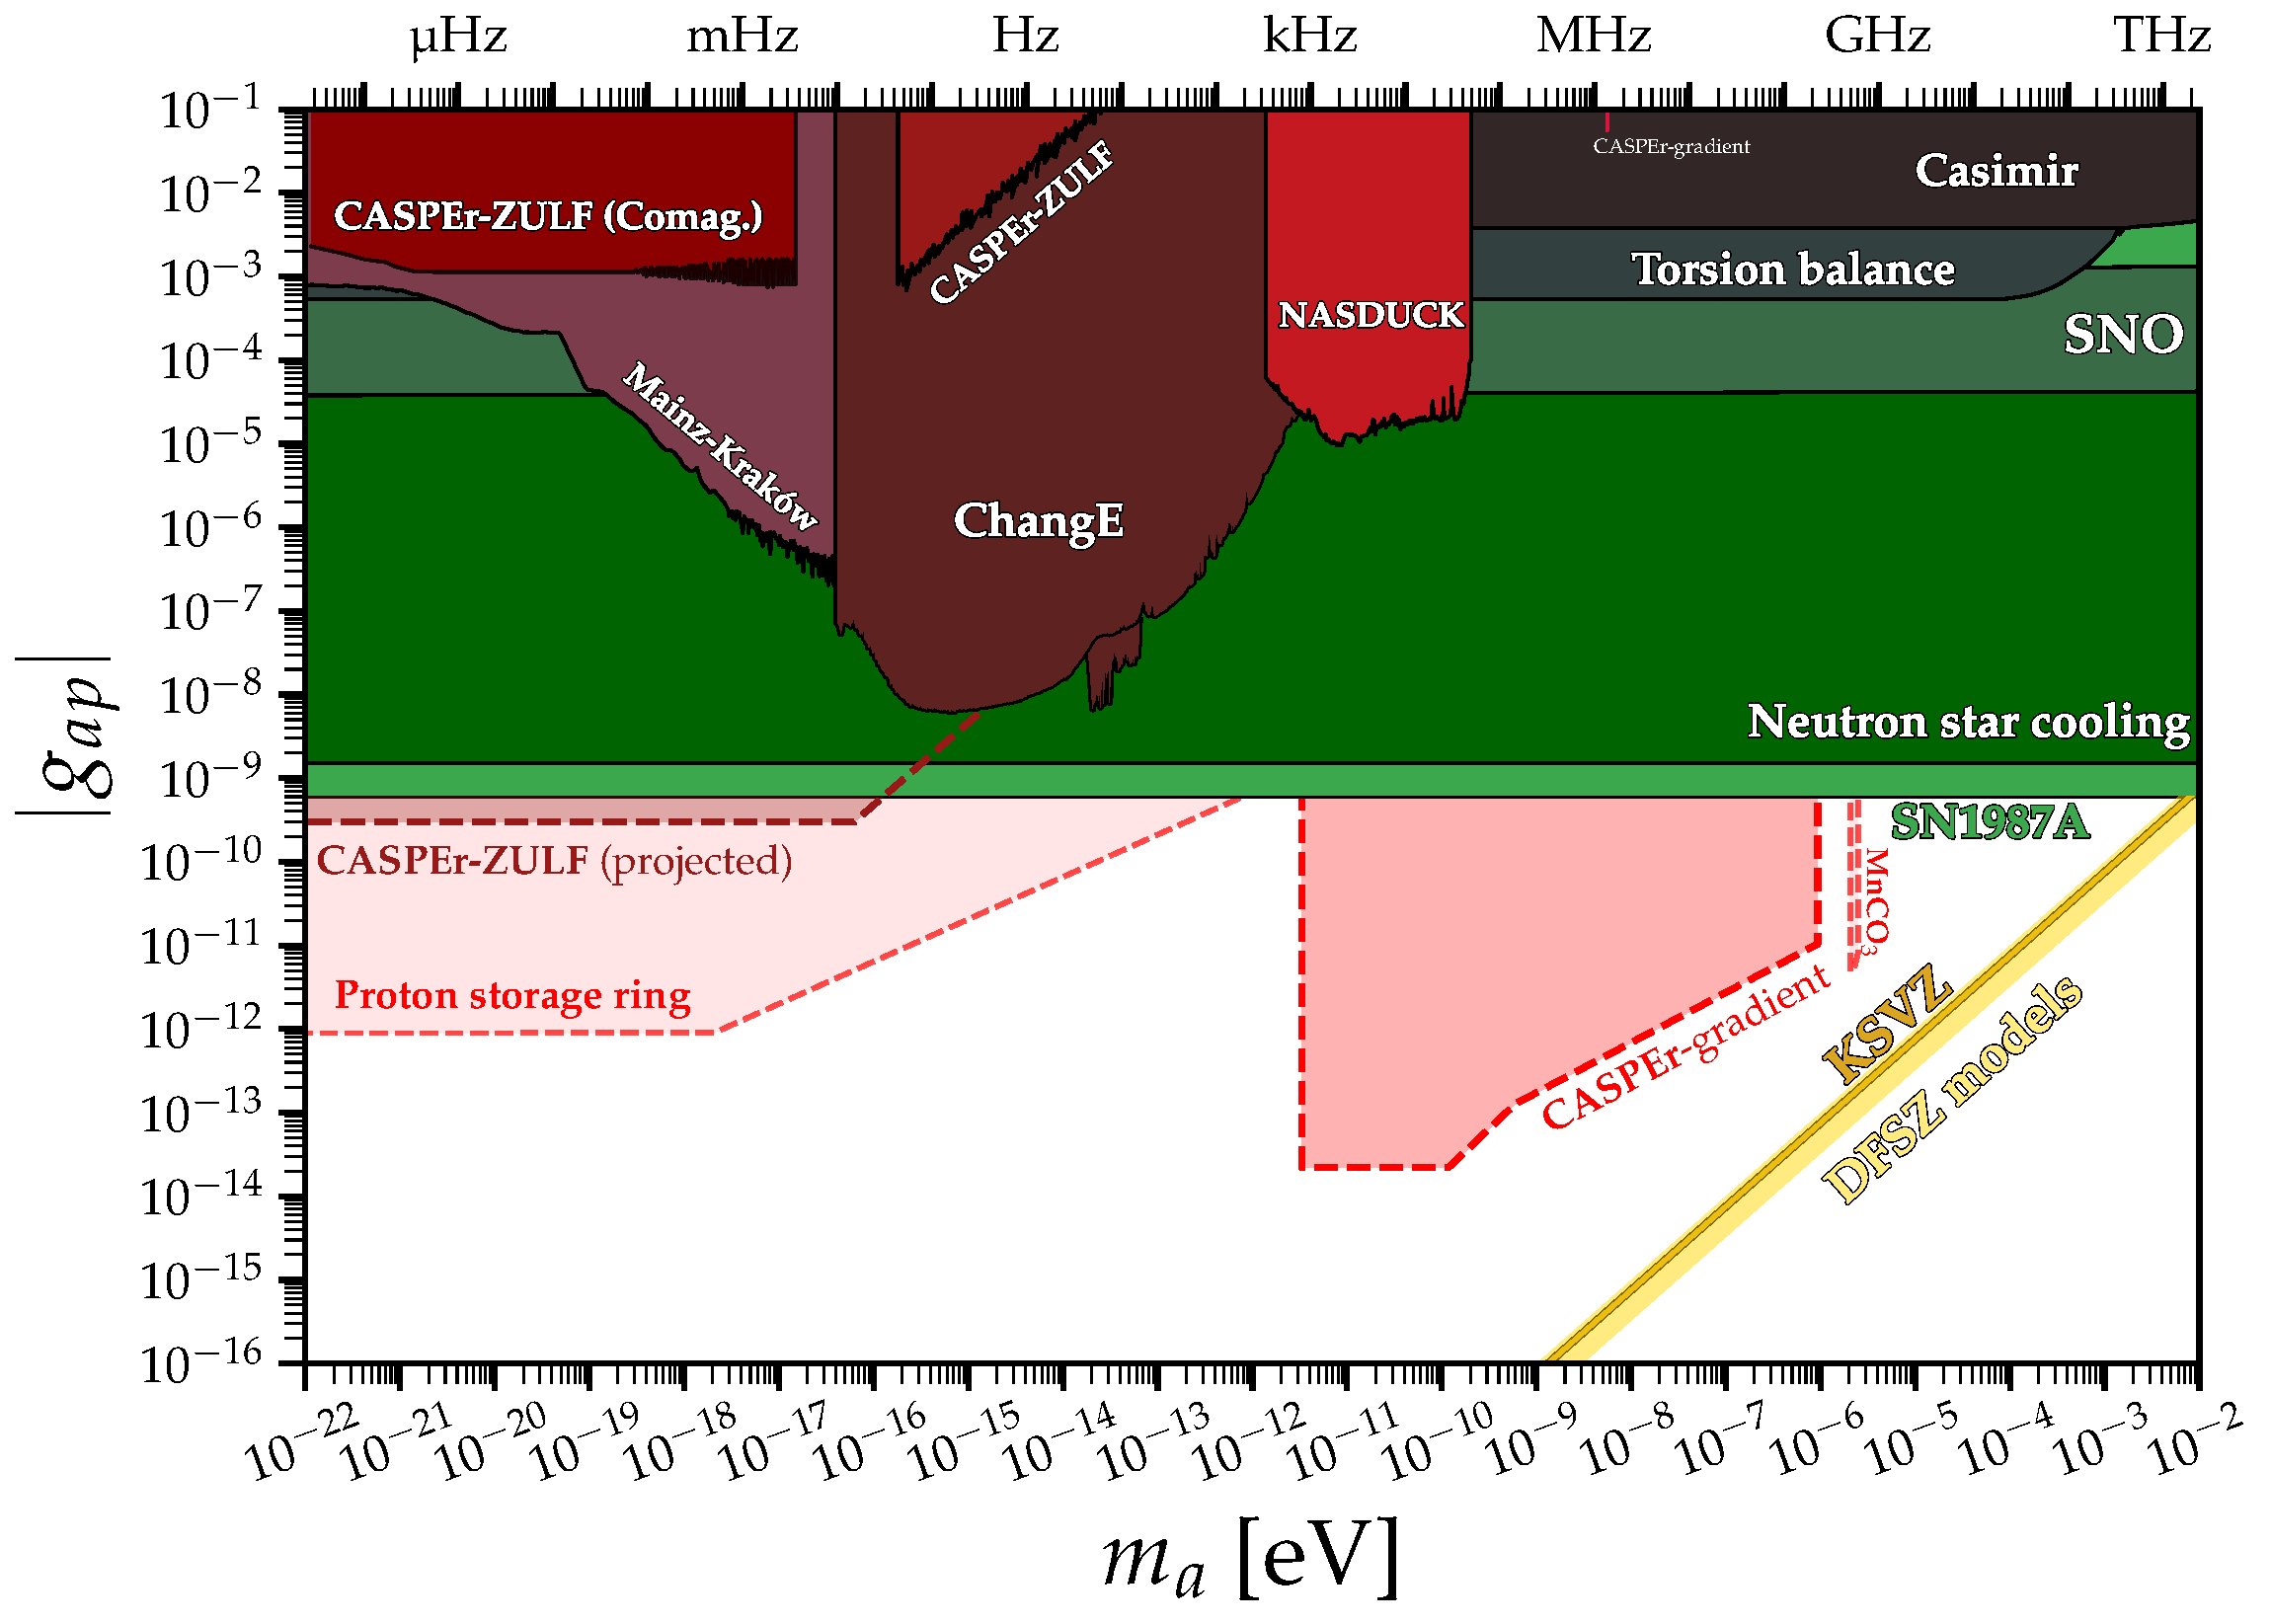
\includegraphics[width=0.99\textwidth]{figures/AxionProton_with_Projections.pdf}
    \caption{ALP-proton mass-coupling parameter space. Solid color blocks represent exclusions. Projections of sensitivities are indicated by the dashed lines on the edges of the blocks. Reproduced from Ref.\,\cite{OHare2020_AxionLimits} with permission.}
\end{figure}


